% ****************************************************************************************************
% Chapter 8: The Safety Framework, Two Paths Compared
% ****************************************************************************************************

\chapter{The Safety Framework: Two Paths Compared}
\label{ch:safety}

The previous chapter ended with an uncomfortable observation. My model achieves a macro F1 of $0.597$ and a Cohen's kappa of $0.701$, matching human inter-rater reliability, but its default decision rule produces an under-triage rate of $15.22\%$. This is three times the maximum rate that the American College of Surgeons Committee on Trauma considers acceptable for clinical deployment. A model that is reliable on average but assigns lower acuity than warranted to one in seven patients is, by that institutional standard, not yet safe.

This chapter is about what can be done to address this. Over approximately three weeks of experiments, I examined three strategies for encoding clinical risk asymmetry into the model's decisions: post-hoc threshold shifting, asymmetric class weights during training, and a custom directional penalty that modifies the loss function to punish under-triage errors more heavily than over-triage errors. All three work to some degree. They do not work the same way, they do not compose, and the relationship between them is the main methodological observation of the chapter.

\section{The Problem in Precise Terms}

Before discussing interventions, I need to be precise about what I am trying to correct.

The model from Chapter~\ref{ch:architecture} produces, for each patient, a probability distribution over the five ESI levels. The default way to turn these probabilities into a discrete prediction is \emph{argmax}: pick the class with the highest predicted probability. This rule is optimal when the cost of every error is the same. In clinical triage, it is not.

\begin{notebox}[Under-triage and Over-triage, Precisely]
\textbf{Under-triage} means predicting a less urgent acuity level than the true level. If a patient is truly ESI-1 and the model predicts ESI-3, that is under-triage: the patient has been assigned to a slower treatment queue than they should be in. Under-triage can kill.

\textbf{Over-triage} means predicting a more urgent acuity level than the true level. If a patient is truly ESI-4 and the model predicts ESI-2, that is over-triage: resources are allocated that the patient did not strictly need. Over-triage wastes resources but rarely causes harm.

The American College of Surgeons Committee on Trauma (ACS-COT) publishes specific tolerances: under-triage should be $\leq 5\%$; over-triage up to $25$--$50\%$ is acceptable. This $10{:}1$ asymmetry is not a statistical convention, it is a clinical policy decision, encoding the judgement that missing a critical patient is an order of magnitude more dangerous than temporarily over-allocating resources to a stable one \citep{acscot2014resources}.

In my setup, under-triage occurs when $\hat{y} > y_{\text{true}}$ (because higher ESI numbers mean lower acuity in the ESI convention). Over-triage occurs when $\hat{y} < y_{\text{true}}$. Severe under-triage means the prediction is off by at least two levels in the dangerous direction.
\end{notebox}

The question I want to ask is not ``can I reduce under-triage?'', of course I can, by simply predicting ESI-1 for everyone. The question is: across all possible decision rules I might apply to this model's probability outputs, what is the best achievable combination of macro F1 and under-triage rate? And within that set of achievable trade-offs, which specific rules come closest to meeting the ACS-COT target?

\begin{notebox}[What Is a Pareto Frontier?]
Suppose you are choosing between strategies that trade off two quantities, in my case, macro F1 (which I want to maximise) and under-triage rate (which I want to minimise). Any given strategy gives you some value of each. Plotting all the strategies as points on a 2D plot, some are clearly worse than others: if strategy A has both higher F1 \emph{and} lower under-triage than strategy B, then B is \emph{dominated} and there is no reason to use it.

The \emph{Pareto frontier} is the set of non-dominated strategies, the outer shell of the point cloud, the ones for which you cannot improve on one dimension without worsening the other. Every rational decision-maker should pick some point on the Pareto frontier. Which point depends on how much you are willing to trade one objective for the other.

In my setting, the Pareto frontier is the operational menu: a list of achievable trade-offs between accuracy and safety. The ACS-COT target specifies one particular demand ($\text{UT} \leq 5\%$), and the frontier tells me what F1 is achievable under that constraint.
\end{notebox}

\section{Strategy 1: Post-hoc Threshold Shifting}

The simplest intervention is also the cheapest. Rather than changing how the model is trained, I change the decision rule applied to its outputs.

Recall from Chapter~\ref{ch:architecture} that my final prediction is not a raw argmax but a \emph{per-class threshold-weighted} argmax:
\[
\hat{y} = \arg\max_c \left( \theta_c \cdot p_c \right)
\]
where $p_c$ is the predicted probability of class $c$ and $\theta_c$ is a class-specific multiplier. Setting $\theta_1 = 2.5$, for example, multiplies the probability of ESI-1 by 2.5 before the argmax, pushing marginal predictions upward. The higher the multiplier on the more urgent classes, the more the model errs on the side of caution.

This is a one-parameter family of decision rules. As the multiplier on the urgent classes increases, under-triage falls, and so does macro F1, because the model is being forced away from its statistically optimal predictions. Sweeping the multiplier produces what clinicians call an \emph{operating curve}: the set of achievable $(F1, \text{UT})$ trade-offs accessible through this intervention.

\begin{figure}[htbp]
 \centering
 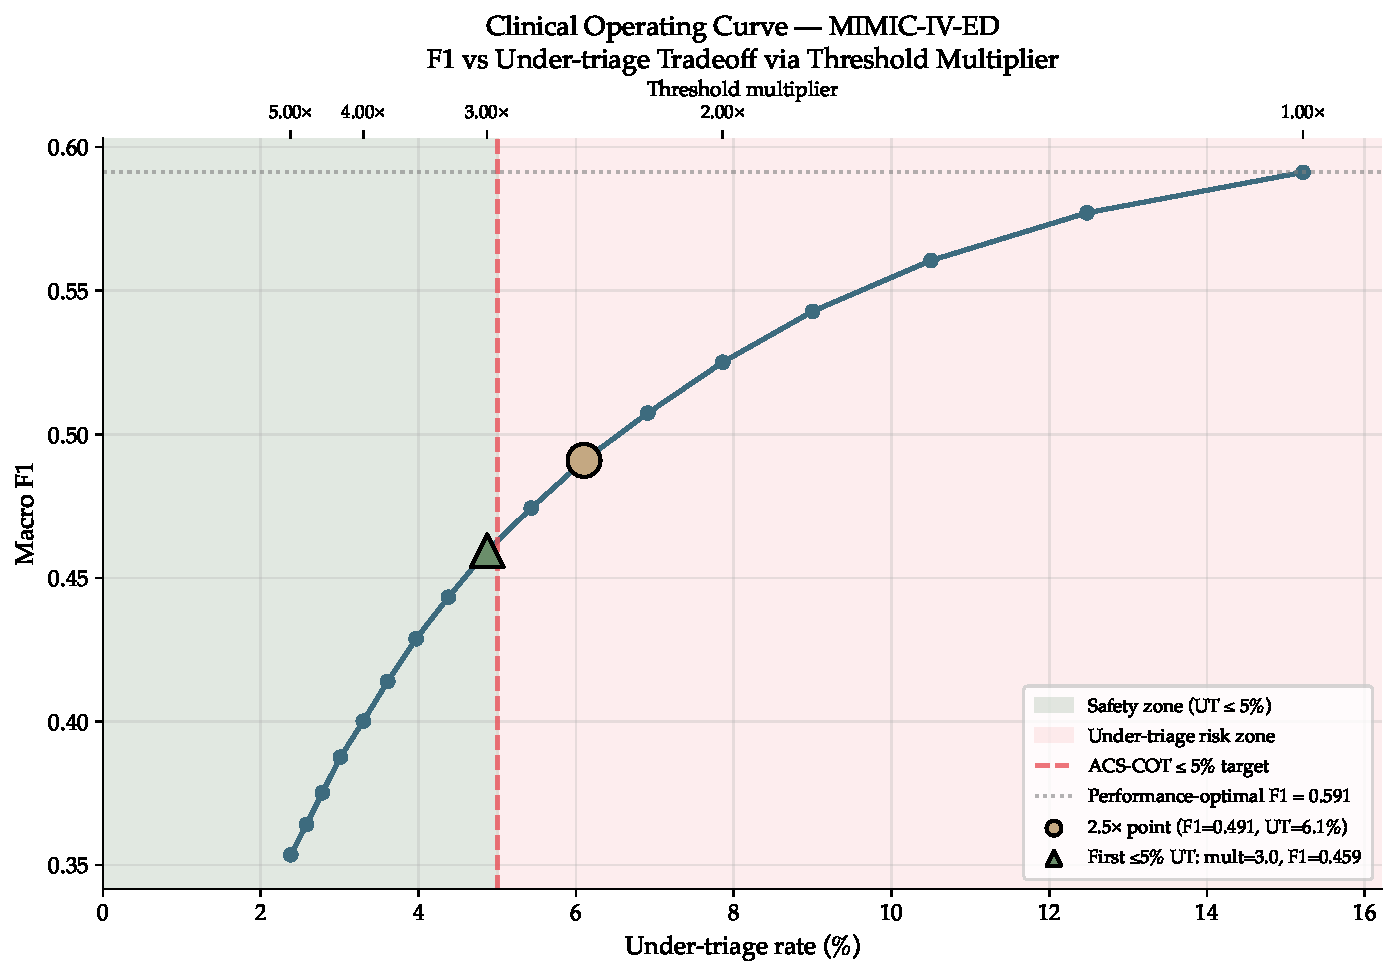
\includegraphics[width=0.9\textwidth]{figures/clinical_operating_curve.pdf}
 \caption[Clinical operating curve]{The operating curve achievable through post-hoc threshold shifting. Each point corresponds to one setting of the threshold multiplier, with the multiplier value labelled on the top axis. At multiplier $1.0$ (right end) I recover the default argmax behaviour: $F1 = 0.591$, $\text{UT} = 15.22\%$. Increasing the multiplier moves leftward and upward on the UT axis: more over-triage, less under-triage. The multiplier $= 3.0$ point, highlighted, is the first that crosses into the ACS-COT safety zone ($\text{UT} \leq 5\%$), but F1 has dropped to $0.459$. The multiplier $= 2.5$ point corresponds to $\text{UT} = 6.1\%$ and $F1 = 0.491$, a less extreme but still substantial compromise.}
 \label{fig:operating-curve}
\end{figure}

The operating curve, shown in Figure~\ref{fig:operating-curve}, is informative in two ways. First, it is smooth and predictable: the trade-off is well-behaved, and I can pick any point along it. Second, it is steep in the range that matters. Moving from $\text{UT} = 15\%$ to $\text{UT} = 6\%$ costs about $0.10$ F1. Moving further down to $\text{UT} = 5\%$ costs another $0.03$. The marginal cost of each additional percentage point of safety increases as I push toward the ACS-COT target, which is what I would expect: I am forcing the model further from its statistical optimum, and the cost of that forcing grows non-linearly.

The first multiplier value at which I meet the ACS-COT $5\%$ under-triage target is $\text{mult} = 3.0$. At that point, F1 is $0.459$. This is the cost of safety through thresholds alone: roughly $0.14$ F1 sacrificed, about a $23\%$ relative reduction in macro F1, to meet the institutional standard.

\begin{notebox}[Why Threshold Optimisation Is Not Retraining]
Post-hoc threshold shifting does not change the model. It changes the rule I apply to the model's outputs. The underlying probability estimates, ``this patient has a $22\%$ chance of being ESI-1'', are unchanged; what changes is the mapping from those probabilities to a discrete prediction.

This distinction matters because of what threshold shifting \emph{cannot} do. It cannot make the model more accurate. It cannot help the model learn patterns it did not learn during training. All it can do is move the decision boundary among the probabilities the model already produces. If the model's probability estimates place a critically ill patient at $15\%$ ESI-1 and $35\%$ ESI-2, no threshold shift can recover the correct prediction without also pushing many non-critical patients into ESI-1. The threshold rule is a re-sorting of the existing probabilities, not a re-estimation of them.

This is why threshold shifting is cheap and fast (seconds to optimise), and also why it has a ceiling on what it can achieve.
\end{notebox}

The ceiling matters. Threshold shifting is useful, but it is applying a correction downstream of a model that was trained with symmetric costs. The natural next question is whether I can do better by making the model aware of the asymmetry during training itself.

\section{Strategy 2: Asymmetric Class Weights}

Gradient-boosted tree libraries and most neural network frameworks support per-class sample weights during training. In the standard setup, each sample contributes equally to the loss. With weights, samples from certain classes contribute more.

For my purposes, the intervention is to increase the weight of the high-acuity classes (ESI-1 and ESI-2), so that errors on those classes count for more during optimisation. A model trained with higher weights on ESI-1 will, other things equal, learn decision boundaries that are less likely to misclassify an ESI-1 patient, in either direction, but with larger effect on the dominant direction of error, which in my case is under-triage from ESI-1 and ESI-2 down to ESI-3.

\begin{notebox}[Cost-Sensitive Learning via Sample Weights]
Cost-sensitive learning is a body of techniques for training classifiers when different types of errors have different costs. The simplest implementation is class-weighted loss: during training, each sample's contribution to the loss function is multiplied by a weight specific to its class.

In the context of gradient-boosted trees, this changes what the trees learn at each split. Instead of optimising predictions to minimise average error across samples, the model optimises to minimise weighted error, where ESI-1 and ESI-2 samples count more. The result is a model whose probability estimates are biased toward flagging high-acuity patients more readily.

Formally, if the weight vector is $w = (w_1, w_2, \ldots, w_5)$ across classes, the training objective becomes
\[
\mathcal{L} = \sum_{i} w_{y_i} \cdot \ell(\hat{y}_i, y_i)
\]
where $\ell$ is the per-sample loss (cross-entropy in my case) and $y_i$ is the true class of sample $i$. Setting $w = (8, 5, 2, 1, 1)$ means ESI-1 errors contribute eight times as much to the gradient as ESI-5 errors. The model's parameters move further to fit those samples.
\end{notebox}

I tested a grid of weight configurations, ranging from mild asymmetry $(2, 1.5, 1, 1, 1)$ through moderate $(3, 2, 1, 1, 1)$ and strong $(5, 3, 1, 1, 1)$ up to heavy $(8, 5, 2, 1, 1)$ asymmetry. For each configuration I retrained the full blend from scratch, a considerably more expensive operation than the threshold sweep, since each configuration requires roughly 40 minutes of CPU time. Table~\ref{tab:asym-weights} presents the key results.

\begin{table}[htbp]
 \centering
 \caption[Asymmetric training weight configurations]{A subset of the asymmetric class weight configurations tested, showing the four Pareto-optimal variants from a sweep of 20 configurations. Each configuration is a vector of weights for classes ESI-1 through ESI-5, applied as sample weights during training. ``F1 (training only)'' is the macro F1 achieved by that weighted model using default argmax; ``UT (training only)'' is its under-triage rate. Heavier asymmetry pushes under-triage down but at a cost in overall F1.}
 \label{tab:asym-weights}
 \small
 \begin{tabular}{lcccc}
 \toprule
 Configuration & Weights (ESI-1 to 5) & F1 & UT & Severe UT \\
 \midrule
 Default (no weighting) & $(1, 1, 1, 1, 1)$ & $0.591$ & $15.22\%$ & $0.57\%$ \\
 Mild+ & $(2, 1.5, 1, 1, 1)$ & $0.560$ & $11.22\%$ & $0.46\%$ \\
 Moderate2 & $(3, 2, 1, 1, 1)$ & $0.554$ & $9.58\%$ & $0.42\%$ \\
 Strong3 & $(5, 3, 1, 1, 1)$ & $0.547$ & $7.73\%$ & $0.38\%$ \\
 Heavy3 & $(8, 5, 2, 1, 1)$ & $0.506$ & $7.44\%$ & $0.36\%$ \\
 \bottomrule
 \end{tabular}
\end{table}

The pattern is clear enough: more aggressive weighting lowers under-triage but at a cost in F1. The heaviest weighting I tried, $(8, 5, 2, 1, 1)$, brings under-triage down to $7.44\%$, closer to the ACS-COT target than the default, but still not meeting it, while sacrificing $0.085$ F1 compared to the default.

No configuration in my sweep reached the $5\%$ under-triage target through training weights alone. The closest was Heavy3 at $7.44\%$, which represents a substantial departure from symmetric training but still falls short of the institutional standard. More extreme weights might push further, but my experiments showed sharply diminishing returns past Heavy3: doubling the weights again produced only marginal additional reductions in under-triage while causing larger F1 losses.

This is the first non-trivial result of the chapter. Asymmetric training weights, applied without post-hoc correction, produce a family of operating points: each weight configuration is one point in F1-vs-UT space. The full set of 20 configurations I tested is plotted in the left portion of Figure~\ref{fig:pareto}, along with the threshold-shifting operating curve for comparison.

\section{The Surprising Finding: The Two Strategies Do Not Compose}

The obvious next experiment is to combine the two strategies. Train with asymmetric weights \emph{and} apply threshold shifting on top. In principle, each strategy addresses a different piece of the problem, training weights shape the probability estimates, threshold shifting adjusts the decision rule applied to those estimates, so combining them should be better than either alone.

It is not.

When I take a model trained with asymmetric weights and apply Nelder-Mead-optimised thresholds, the optimisation moves the decision rule back toward the unweighted default. The under-triage rate rises, the F1 rises along with it, and the final operating point lands on almost exactly the same operating curve that threshold shifting alone would have produced from the default-weighted model.

I observed this pattern consistently across weight configurations. Table~\ref{tab:substitute} reports three representative cases.

\begin{table}[htbp]
 \centering
 \caption[Combining training weights with threshold optimisation]{The combined effect of asymmetric training weights and post-hoc threshold optimisation. For each of three training strategies, I report F1 and UT both before and after Nelder-Mead threshold optimisation. In every case, threshold optimisation moves the operating point back toward the default-weighted model's operating curve, the safety gains from asymmetric training are largely undone.}
 \label{tab:substitute}
 \small
 \begin{tabular}{lcccccc}
 \toprule
 & \multicolumn{2}{c}{Training only (argmax)} & \multicolumn{2}{c}{After threshold opt.} & \multicolumn{2}{c}{Net change} \\
 \cmidrule(lr){2-3} \cmidrule(lr){4-5} \cmidrule(lr){6-7}
 Strategy & F1 & UT & F1 & UT & $\Delta$F1 & $\Delta$UT \\
 \midrule
 Default (no asymmetry) & $0.591$ & $15.22\%$ & $0.597$ & $14.50\%$ & $+0.006$ & $-0.72$pp \\
 Moderate asym. weights & $0.547$ & $7.73\%$ & $0.578$ & $15.38\%$ & $+0.031$ & $+7.65$pp \\
 Directional penalty & $0.475$ & $6.80\%$ & $0.558$ & $15.50\%$ & $+0.083$ & $+8.70$pp \\
 \bottomrule
 \end{tabular}
\end{table}

The pattern is not subtle. Moderate asymmetric weights produce a model at $\text{UT} = 7.73\%$; after threshold optimisation, it settles at $\text{UT} = 15.38\%$. The directional penalty approach (which I describe in detail below) produces a model at $\text{UT} = 6.80\%$; after threshold optimisation, it settles at $\text{UT} = 15.50\%$. The under-triage reductions from training are almost completely reversed.

The interpretation is straightforward once I see it clearly. Both strategies are working on the same underlying quantity, the discrepancy between the statistically optimal decision boundary and the clinically safe decision boundary. Asymmetric training weights bias the probability estimates so that argmax lands closer to the safe boundary. Threshold shifting adjusts the decision boundary without touching the probabilities. When both are applied, the threshold optimiser's job is to find the boundary that maximises the chosen objective (in the table above, macro F1), which means reversing whatever the asymmetric training did to shift the probabilities.

The two strategies are not additive. They are substitute mechanisms for the same correction, and the correction cannot be applied twice. Once a decision rule has been calibrated to the chosen F1-UT trade-off, it does not matter whether the calibration was baked into training or applied post-hoc, the resulting operating point is the same.

\begin{remarkbox}[Why This Matters]
The substitute-not-complementary finding has practical consequences for anyone designing a clinical ML system. The natural instinct, when facing a safety constraint, is to reach for every available lever: weight the training loss, adjust the thresholds, maybe add an ordinal penalty for good measure. But if all these levers operate on the same decision boundary, stacking them is at best wasted effort and at worst a way of obscuring what the model is actually doing.

The practical recommendation is: pick one. If the clinical risk asymmetry is known before training, it can be encoded as sample weights, producing a model whose raw argmax output is already appropriately conservative. If the asymmetry needs to be configurable at deployment time, if different hospitals might want different operating points, then train a standard model and use threshold optimisation, which can be recomputed in seconds for any desired operating point. But do not do both and expect them to compound.

I prefer the threshold-optimisation path because it is transparent, fast, and configurable. A hospital can inspect the decision rule (``predict ESI-1 whenever $2.5 \cdot p_1$ exceeds every other $p_c$'') and choose their own trade-off by choosing their own multiplier. A model with baked-in asymmetric training is a black box in this regard, its probability outputs are already biased, and understanding what operating point they correspond to requires re-analysing the trained model.
\end{remarkbox}

\section{Strategy 3: The Directional Ordinal Penalty}

Before settling on the substitute interpretation, I ran one more experiment. If simple class weights are just another way of adjusting the decision boundary, what about an approach that modifies the training loss more fundamentally, one that penalises different directions of error differently?

This is the directional ordinal penalty. Rather than weighting by class, I weight by the direction of the error. Under-triage errors (predictions that are less urgent than the true label) incur a loss multiplier larger than the default; over-triage errors (predictions more urgent than warranted) incur a smaller multiplier. The magnitude of the asymmetry encodes the clinical priority: with a factor of 10, for example, the loss for predicting ESI-3 when the truth is ESI-1 is ten times the loss for predicting ESI-1 when the truth is ESI-3.

Implementing this for gradient-boosted trees required a custom sample weight scheme computed on-the-fly based on the model's current predictions. I implemented it within LightGBM's training loop and tested several asymmetry factors.

The approach works, in the narrow sense that it substantially reduces under-triage. The best configuration (Variant C in the summary plots below) achieved $\text{UT} = 6.80\%$ with F1 $= 0.475$ before any threshold adjustment. This is a steeper F1 cost than the asymmetric class weights, the loss modification is more aggressive, but the under-triage reduction is also slightly larger in absolute terms.

Figure~\ref{fig:ordinal-penalty} shows all three training strategies compared head-to-head, both with and without post-hoc threshold optimisation.

\begin{figure}[htbp]
 \centering
 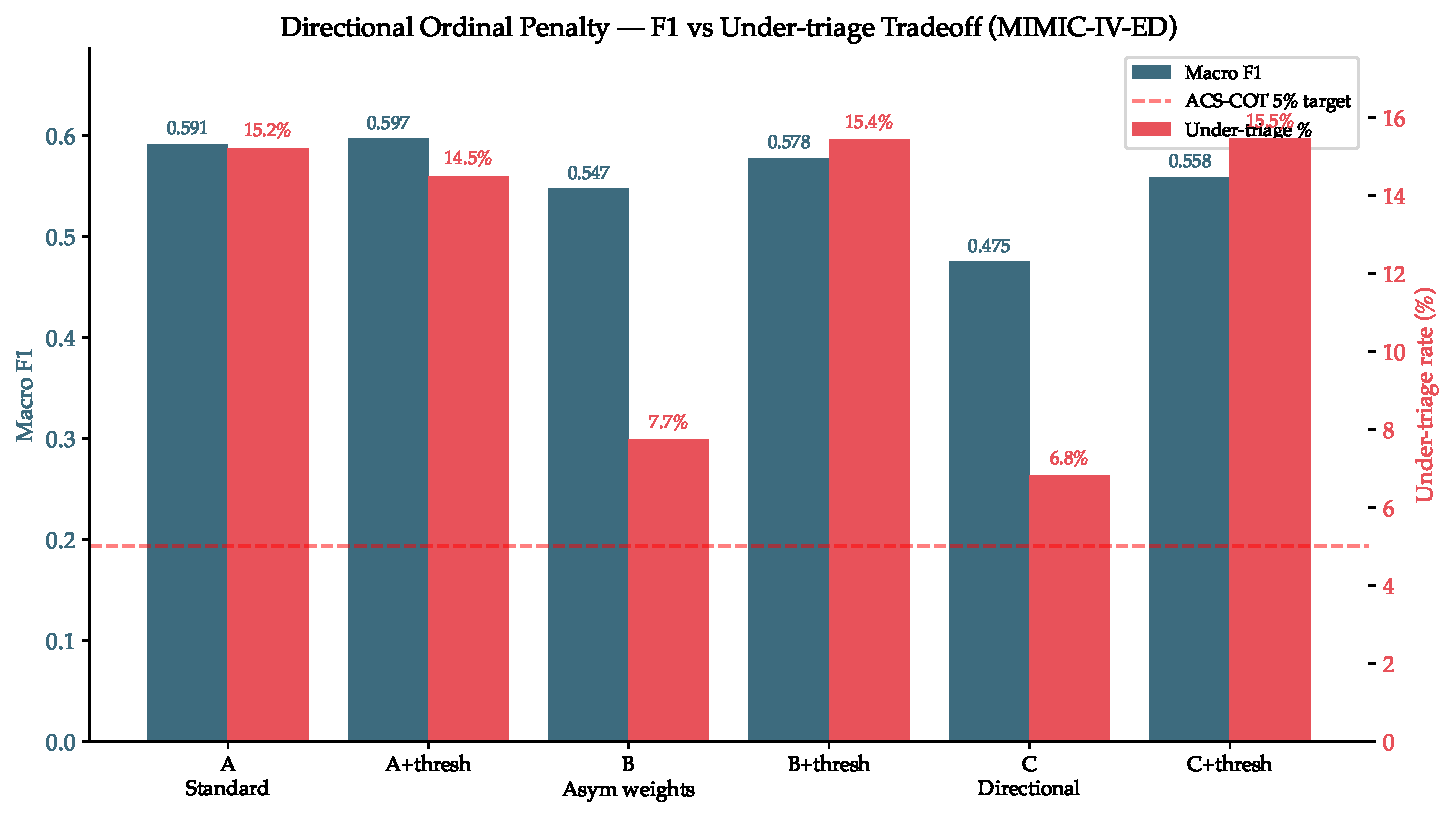
\includegraphics[width=0.95\textwidth]{figures/ordinal_penalty_comparison.pdf}
 \caption[Three training strategies compared, with and without threshold optimisation]{Macro F1 (blue, left axis) and under-triage rate (red, right axis) for three training strategies, each shown before and after post-hoc threshold optimisation. Variant A is the default blend; Variant B uses asymmetric class weights; Variant C uses the directional ordinal penalty. Without threshold optimisation (A, B, C), the three strategies occupy distinct points in F1-UT space, with more aggressive training producing lower UT at lower F1. After threshold optimisation (A+thresh, B+thresh, C+thresh), all three converge toward a similar operating point around $\text{UT} \approx 15\%$ and $F1 \approx 0.58$--$0.60$. The safety benefits of the more aggressive training strategies are almost entirely undone by the post-hoc optimiser.}
 \label{fig:ordinal-penalty}
\end{figure}

This figure makes the substitute finding inescapable. The three bars on the left side of each pair (A, B, C) show three genuinely different operating points, the training interventions work. The three bars on the right side (A+thresh, B+thresh, C+thresh) show that the threshold optimiser, given the objective of maximising F1, unwinds almost all of the asymmetry and lands the three models in a narrow band around $15\%$ under-triage.

The per-class F1 breakdown is even more revealing. Figure~\ref{fig:per-class-strategies} shows the F1 score for each ESI class under the three training strategies (before threshold optimisation).

\begin{figure}[htbp]
 \centering
 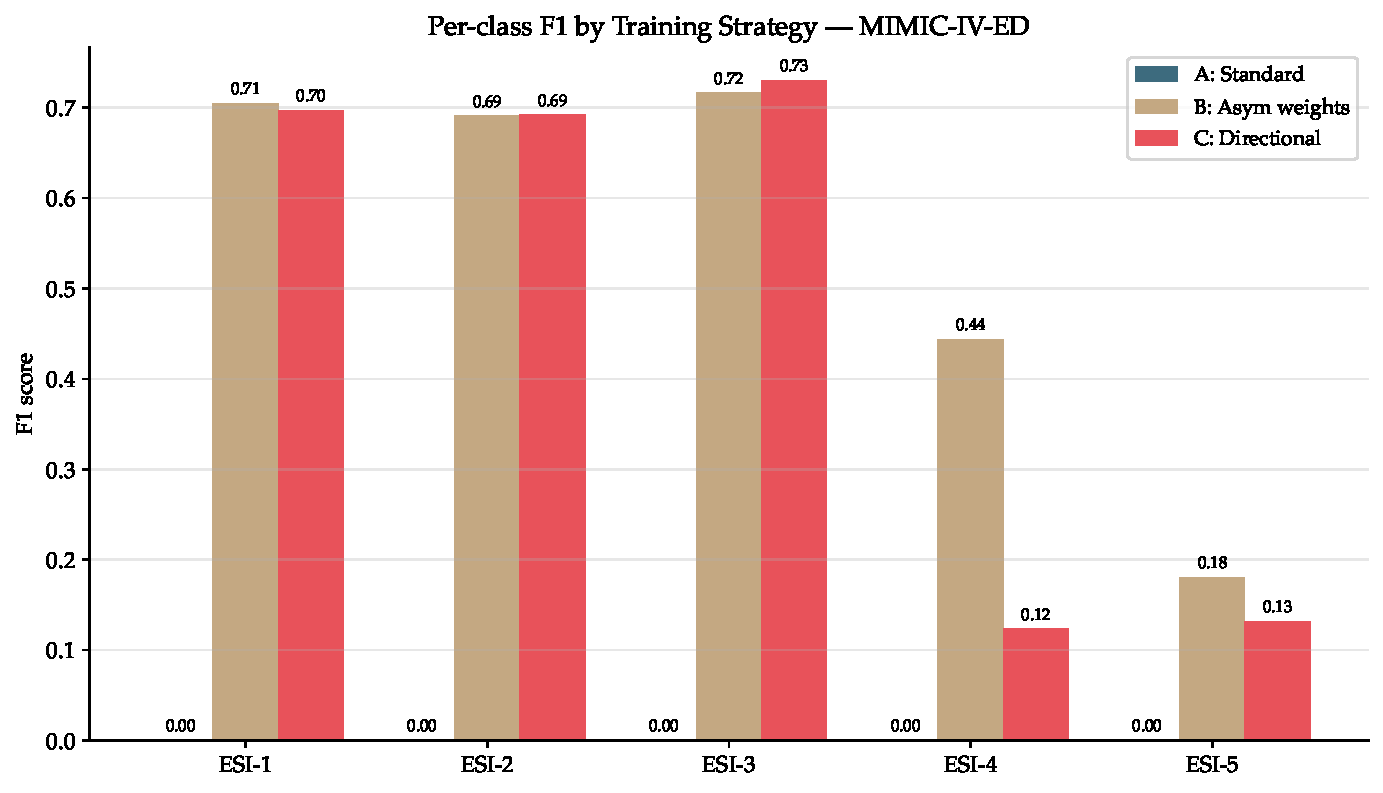
\includegraphics[width=0.9\textwidth]{figures/per_class_f1_comparison.pdf}
 \caption[Per-class F1 under three training strategies]{F1 score for each ESI class under the three training strategies, before threshold optimisation. The standard blend (Variant A, not shown here because it serves as the baseline with $\text{F1} > 0$ for all classes) achieves $0.70$/$0.69$/$0.77$/$0.54$/$0.26$. Asymmetric weights (B, gold) preserve performance on the high-acuity classes at a cost to ESI-4 and particularly ESI-5. The directional penalty (C, red) is more aggressive: it preserves ESI-1/2/3 performance but sacrifices ESI-4 ($0.12$) and ESI-5 ($0.13$) dramatically. This is the trade-off made visible: aggressive safety training concentrates errors in the lower-acuity classes where those errors are clinically less costly.}
 \label{fig:per-class-strategies}
\end{figure}

The per-class view shows where the safety-oriented training strategies pay their cost. Variants B and C both preserve F1 on ESI-1, ESI-2, and ESI-3, the high- and mid-acuity classes, while sacrificing performance on ESI-4 and especially ESI-5. This is exactly the trade-off the clinical risk asymmetry calls for: errors on ESI-4 and ESI-5 (``I thought this patient needed a lab test and actually they didn't'') are clinically minor, while errors on ESI-1 and ESI-2 (``I thought this patient was stable and actually they were critical'') can be catastrophic. The safety-trained models are telling me something sensible: accept more noise in the low-acuity end of the scale in exchange for more reliable identification of the truly sick.

\section{Putting It All Together: The Pareto Frontier}

I now have enough pieces to construct the full picture. For any given target under-triage rate, what is the best F1 I can achieve, across all the strategies I have tested?

Figure~\ref{fig:pareto} is the answer, and summarises much of the chapter.

\begin{figure}[htbp]
 \centering
 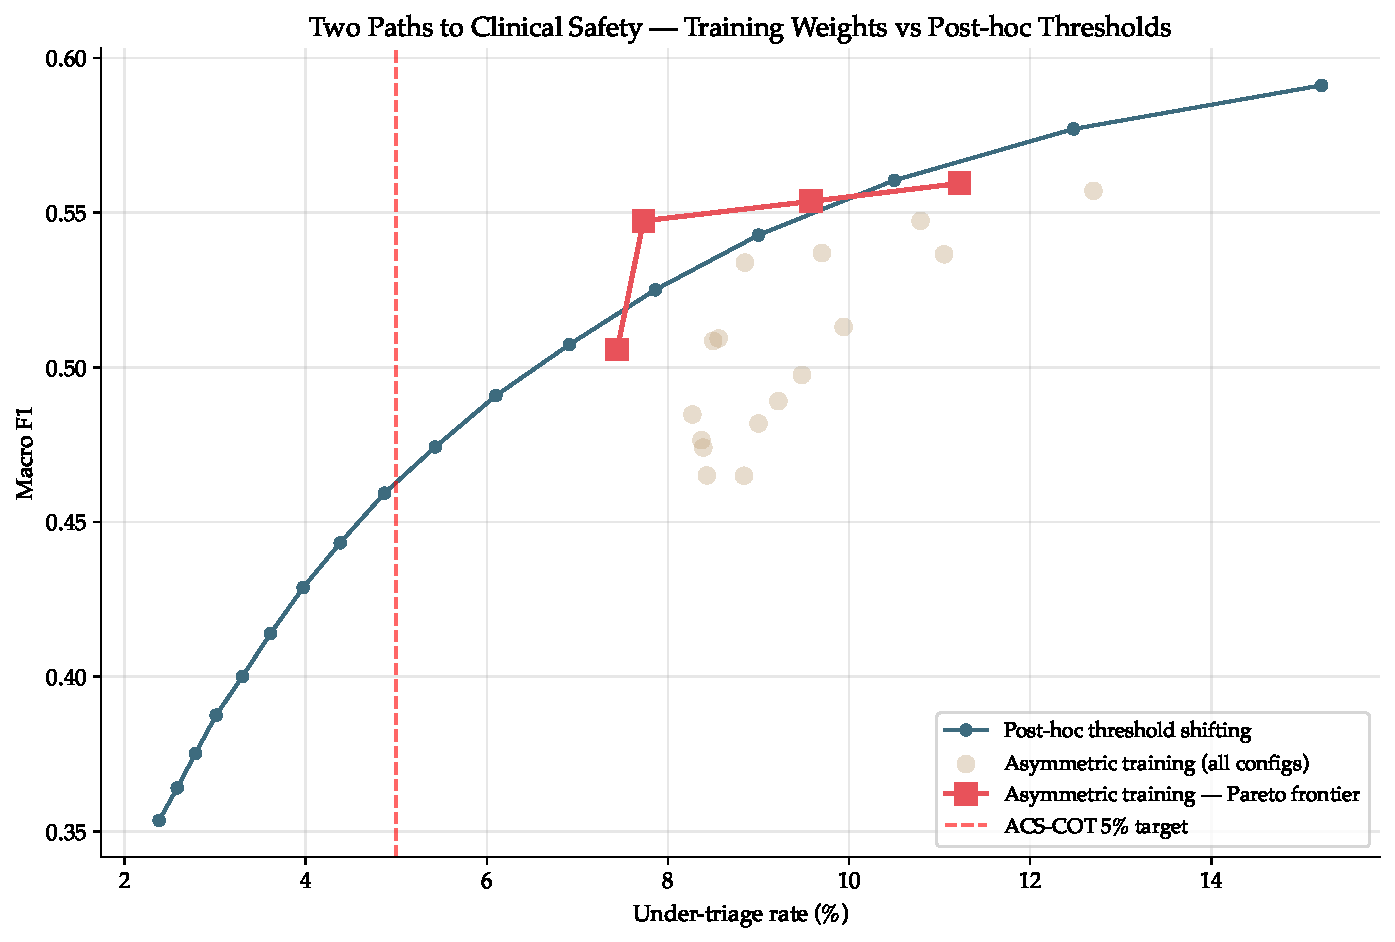
\includegraphics[width=\textwidth]{figures/pareto_training_vs_threshold.pdf}
 \caption[Pareto frontier: training weights vs threshold shifting]{The achievable operating points for my model, plotted as macro F1 (y-axis) against under-triage rate (x-axis). Blue curve: post-hoc threshold shifting applied to the default blend, producing a smooth operating curve. Gold circles: the 20 asymmetric class-weight configurations I tested, each a separately-trained blend. Gold squares with red outline: the four Pareto-optimal weight configurations from the gold-circle cloud. Red dashed line: the ACS-COT $5\%$ under-triage target. The threshold-shifting curve and the asymmetric-weights Pareto frontier track each other closely across the range that matters. In the clinically relevant region ($\text{UT} < 12\%$), threshold shifting consistently reaches the same F1 or slightly better than the corresponding asymmetric-weights configuration.}
 \label{fig:pareto}
\end{figure}

The figure has three components. The blue curve is the operating curve from post-hoc threshold shifting on the default-weighted model. It spans $\text{UT} = 15.2\%$ (multiplier $1.0$) down to $\text{UT} \approx 2.4\%$ (multiplier $5.0$), with F1 decreasing monotonically from $0.591$ to $0.354$. The gold circles are each of the 20 asymmetric weight configurations, each produced by a separate full model training. The gold squares with red outlines are the Pareto-optimal subset: the four weight configurations that are not dominated by any other.

The central observation is that the blue curve and the gold squares track each other closely. In the region where the ACS-COT target lives, $\text{UT}$ between $5$ and $12\%$, the threshold-shifting curve consistently matches or slightly beats the asymmetric-weights frontier. Every asymmetric weight configuration I trained can be matched or exceeded by a threshold multiplier on the default-weighted model.

This is the operational consequence of the substitute-not-complementary finding. Since the two strategies produce essentially the same frontier of achievable trade-offs, there is no reason to prefer the more expensive approach. Threshold shifting is fast, interpretable, and can be recomputed for any desired operating point without retraining. Asymmetric training is slow, opaque, and bakes a particular operating point into the model.

\section{Does Anything Meet the ACS-COT Standard?}

Yes, but at a cost.

Looking at the blue curve in Figure~\ref{fig:pareto}, the first point that crosses the ACS-COT $5\%$ under-triage threshold is threshold multiplier $3.0$, which yields $\text{UT} = 4.87\%$ at $\text{F1} = 0.459$. A slightly more aggressive configuration, isotonic-calibrated probabilities with multiplier $3.25$, reaches $\text{UT} = 4.96\%$ at $\text{F1} = 0.440$. (Isotonic calibration is discussed in Chapter~\ref{ch:calibration}; the short version is that it re-fits the model's probability outputs to be better-calibrated, which nudges the operating curve slightly.)

Either way, meeting the ACS-COT standard requires accepting a macro F1 of approximately $0.44$--$0.46$. This is $0.13$--$0.15$ lower than the unconstrained optimum of $0.597$, a relative reduction of roughly $25\%$.

\begin{notebox}[Decision Curves in Clinical ML]
A common theme in clinical machine learning is that there is no ``correct'' operating point that a researcher can recommend. The choice depends on the hospital's resources, the population they serve, and their tolerance for different types of errors.

My job, as the developers of the model, is to make the trade-off legible. I publish the full operating curve, I explain what each point on it means clinically, and I describe the sensitivities. The hospital implementing the system can then choose the point that makes sense for their context.

A rural critical-access hospital with a single triage nurse on a night shift might value the $\text{UT} \leq 5\%$ target heavily and accept the $\text{F1} = 0.46$ trade-off, because over-triage there is cheap (send the patient to a bed) and under-triage is catastrophic (no immediate backup). A tertiary academic medical centre with five triage nurses, a full resident team, and abundant resources might value F1 more highly, preferring the multiplier $1.0$ operating point and managing safety through redundant human review.

Both choices are defensible. The right role for the ML system is to support both, not to impose one.
\end{notebox}

I do not recommend a specific operating point in this report. My view is that the choice of operating point is a clinical policy decision, not a technical one. What I can offer is the curve itself and the evidence that it is a tight Pareto frontier, you really do have to give up F1 to buy safety, and the exchange rate is roughly $0.02$ F1 per percentage point of under-triage reduction in the clinically relevant range.

\section{The Structural Finding}

Why does the operating curve have this particular shape, and why is it so hard to escape? I think there are two underlying reasons.

The first is that the probability estimates from the model are approximately calibrated. When the model says a patient has $22\%$ probability of being ESI-1, that patient really is ESI-1 about $22\%$ of the time. This means that the Bayes-optimal decision rule (minimising any cost-weighted combination of errors) is essentially just a threshold applied to these probabilities. Different cost structures correspond to different thresholds. There is no additional structure beyond this that the ML system can exploit, the probabilities already summarise everything the model has learned.

The second is that the features available at triage simply do not support $5\%$ under-triage. The data I have, vitals, chief complaint, demographics, prior history, are noisy proxies for acuity. Some critically ill patients present with normal vitals (the compensated shock phenomenon I explore in Chapter~\ref{ch:fairness}). Some mildly ill patients present with alarming complaints. No amount of model engineering can compensate for irreducible uncertainty in the input. To push the under-triage rate down to $5\%$, the model has to over-triage aggressively, which means sending many stable patients to the high-acuity queue. This is not a bug of my method; it is a structural property of the problem.

This matters because it shapes the kind of claim the project can make. I am not saying ``my model can be safely deployed at $5\%$ under-triage'', the evidence suggests that no model trained on these features alone could be deployed at that threshold without unacceptable F1 loss. I am saying ``my model produces a transparent operating curve, and institutions can choose their own point on it.'' The difference is important, and it is one I carry into the rest of the report.

\section{What This Chapter Contributes}

To summarise the chapter's findings:

\begin{itemize}
 \item The default argmax decision rule produces $\text{UT} = 15.22\%$, three times the ACS-COT target. The asymmetric clinical cost structure demands a different decision rule.
 \item Three strategies for encoding the asymmetry were tested: post-hoc threshold shifting, asymmetric class weights during training, and a directional ordinal penalty in the loss function.
 \item All three strategies can reduce under-triage, at a cost in macro F1. The trade-off curves for all three overlap in the clinically relevant range.
 \item The three strategies are substitute, not complementary. Combining them does not compound their effects; the post-hoc threshold optimiser unwinds whatever safety-oriented training did.
 \item For practical deployment, post-hoc threshold shifting is preferable: it is transparent, fast, and configurable at deployment time without retraining.
 \item No configuration I tested meets the ACS-COT $5\%$ under-triage target without substantial F1 loss ($0.13$--$0.15$ reduction from the unconstrained optimum).
 \item This appears to be a structural property of the problem, a consequence of irreducible uncertainty in the triage features, rather than a failure of the methods I tried.
\end{itemize}

The next chapter takes up a different dimension of the evaluation: fairness. The overall operating point conceals substantial variation across patient subgroups, and an intersectional bias audit surfaced a pattern I did not expect, that age, not race, is the larger axis of variation in the model's errors on this cohort, with young patients presenting apparently normal vital signs (the clinical phenomenon of compensated shock) offering a plausible mechanism. That chapter turns from aggregate metrics to subgroup analysis, and raises a question that this chapter's operating curve cannot answer: does moving along the Pareto frontier help everyone equally, or does it help some populations more than others?
